
The limited memory BFGS algorithm (L-BFGS) approximates the inverse Hessian (denoted by $H$) using $m$ past updates of the position and the gradient at the position. These updates are used to implicitly approximate the inverse Hessian. In contrast to the BFGS algorithm, BFGS approximates the Hessian matrix, as opposed to the inverse Hessian.


Similar to the BFGS algorithm, we define
\begin{align*}
    s_k &= x_{k+1} - x_k\\
    y_k &= \nabla f(x_{k+1}) - \nabla f(x_k).
\end{align*}
We also define $\rho = \frac{1}{y_k^Ts_k}$. The update for the inverse Hessian is given as
\[H_{k+1} = (I - \rho_ks_ky_k^T)H_k(I - \rho_ky_ks_k^T) + \rho_ks_ks_k^T\]
For the low-storage aspect, we define a sequence of vectors $q_{k-m}, \dots, q_k$ at a fixed $k$ to be $q_k = \nabla f(x_k)$ and $q_i = (I - \rho_iy_is_i^T)q_{i+1}$. Define another sequence of vectors $z_{k-m},\dots, z_k$ as $z_i = H_iq_i$. The value of $z_k$ is said to be an ascent direction. The L-BFGS algorithm is then given as follows:
\begin{figure}[H]
    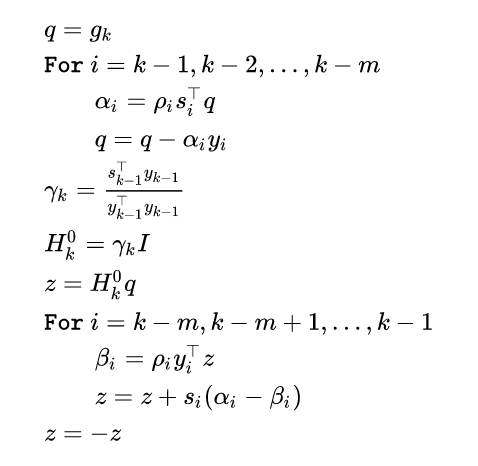
\includegraphics[scale = 1]{images/L-BFGS-Algorithm.png}
    \centering
    \caption{Outline of the L-BFGS algorithm. Taken from Wikipedia.}
\end{figure}
Where $g_k = \nabla f(x_k)$.
\newline
This gives a search direction for the minimization problem.